
%-------------------------------------------------------------------------
\SubSection{Vicon MX motion capture system}

Vicon MX motion capture system is a passive optical system that uses markers
coated with a retroreflective material to reflect light back that is generated near the cameras lens.
The camera's threshold can be adjusted so only the bright reflective markers will be sampled, ignoring skin and fabric.

An object with markers attached at known positions is used to calibrate the cameras and obtain their positions and the lens distortion of each camera is measured. Providing two calibrated cameras see a marker, a 3 dimensional fix can be obtained.

Our system used for this project mainly consists of:

\begin{itemize}
\item 8 Vicon MX3+ cameras, fitted with sensitive solid-state
sensors, with stringent checks for linearity, sensitivity, and absence of jitter.
Each MX camera is programmed with firmware to control its operation
and enable it to perform its own onboard grayscale processing.
Cameras and their relevant characteristics are recognized immediately when they are plugged in to Vicon MX system.

\item MX Ultranet, that supplies power, synchronization, and
communications for all eight connected MX cameras. Only MX Ultranet is connected to the Host PC
and routes all communication to and from the host PC, and timing/synchronization signals to and from the
MX cameras connected to it.

\item Host PC, with separate Ethernet port (preferably Gigabit ethernet card) to enable communications between
the Vicon software installed on this \emph{host pc} (in our case \emph{Vicon IQ 2.5}) and \emph{MX Ultranet}.
No other special requirements for Host PC, but processor and memory are vital for being able to achieve better results. Our \emph{host pc} had 2.49GB of RAM and 1.60GHz Intel Xeon 8 core processor.
\emph{Vicon IQ} software on a \emph{host pc} is used to collect
and process the raw video data. It takes the two-dimensional data from each
camera, combining it with calibration data to reconstruct the equivalent digital
motion in three dimensions. This can be viewed as a virtual
three-dimensional motion. After this reconstruction the data may be passed to
other applications.
\end{itemize}

\begin{figure}
  \centering
  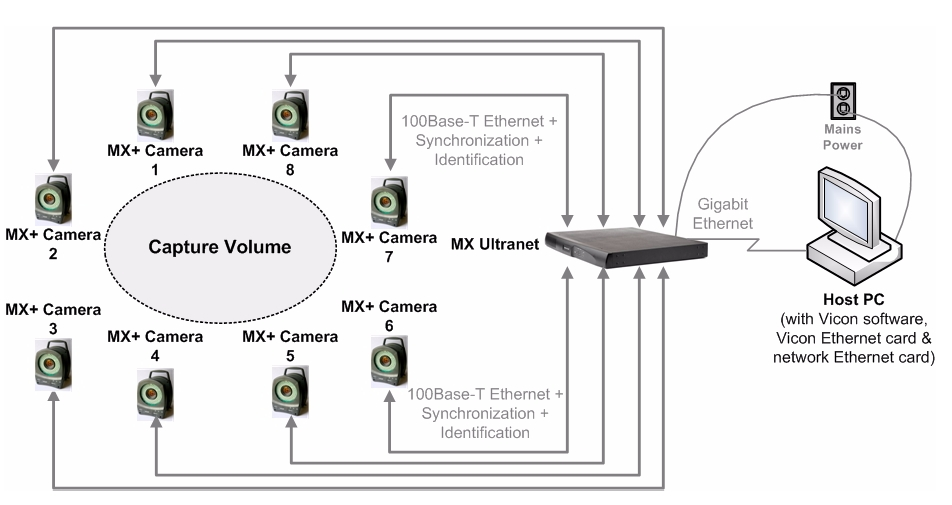
\includegraphics[width=98mm]{images/vicon_mx_basic.jpg}
\end{figure}

%-------------------------------------------------------------------------
\SubSection{Motion system preparations}

Vicon motion capture system high-resolution cameras are situated in a circle,
above the maximum height of any marker that would be captured,
that forms a motion capture space. Then the capture volume is created.
The capture volume is three-dimensional, but in practice is more readily viewed
by its boundaries marked out on the floor. This gives you a guide for the
positioning of the cameras, and your subjects a guide as to where they
can move. The area should be as central to your capture space as possible
to maximize the volume you are able to capture.
Initially you are looking to see whether the camera is positioned and oriented
for the maximum view. Then every single camera can be adjusted separately
by changing software settings, to achieve best result.

After setting up cameras, the vital thing is system calibration.
It allows the software to calculate the relative location and
orientation of all the cameras. When your movements have been recorded the
reconstruction process uses these measurements to calculate the accurate
movements of the markers through space.

This is done by static and dynamic calibrations:

\begin{itemize}
\item Static calibration - calculates the origin or center of the capture volume and determines the
orientation of the 3D Workspace.
\item Dynamic calibration - involves movement/waving of a calibration wand throughout the whole volume and
allows the system to calculate the relative positions and orientations of the
cameras. It also linearizes the cameras.
\end{itemize}

%-------------------------------------------------------------------------
\SubSection{Capturing motion data}

Having the whole motion system ready for use, the next first step is placing all the retroreflective markers on special suit.
The special suit is used to achieve the most accurate results in motion, that motion system gets by tracking those reflective markers and it should be as as tight as possible. Though the suit is not always used while capturing motion data, as for example capturing face motion data, special reflective markers are used, that are put directly on subjects face. Placing markers is vital that the animating template is already selected. In this case, skeleton template, that will be assigned with motion data points. These templates describes the bone structure, joint positions and markers positions, how these markers relate to the bone structure and joints.

When markers are ready, it's time to start capturing data. Motion capture subject should stand in the middle of the circle in the capture area, with his back straight, arms straight out with palms facing down, and feet forwards.
This is called a T-pose, and every capture session should begin and end every in it. This pose is common in animating human bodies, as it allows meshes of the skin to be connected correctly. Also it usually allows the motion capture system to determine all the markers positions right from the frame 1, as all of them are in its visibility area.
While capturing, you should be aware, that during whole capture process, you should be in cameras capture area.

%-------------------------------------------------------------------------
\SubSection{Captured data post-processing}

After capturing motion data, in order to proceed further, post-processing must be done.
Firstly it involves labeling/matching each marker from captured data to our used animation template (skeleton template) at the first frame.
Only by labeling these markers, we are getting logical motion data in further frames, and not some meaningless points in the 3D world. This is the stage, when it's necessary that those reflective markers were situated correctly on the motion capture subject.

Though labeling does really big part in getting correct motion data, it's very important to do some manual tweaking of the labeled points and track unlabeled ones. They can be unlabeled either of some motion capture failure at some point or there can be a "ghost" points that needs to be deleted. Ghost points are quite common while using passive optical motion capture system with retroreflective markers.

\begin{figure}[H]
  \centering
  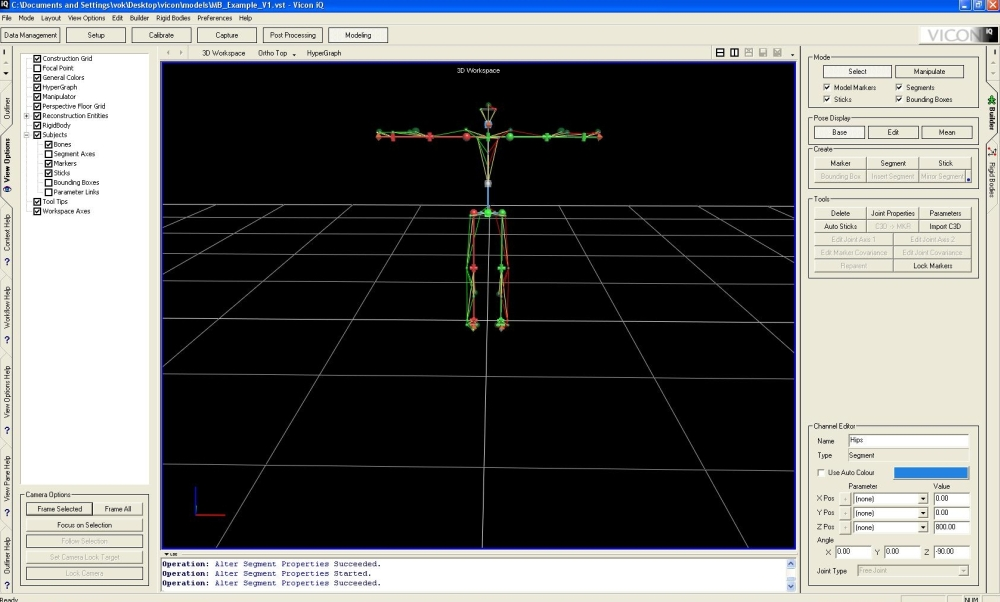
\includegraphics[width=90mm]{images/vicon.jpg}
\end{figure}

Without manual fixing, special pipelines are used to automate various processes, for example using kinematic fitting to match our animation template to our labeled markers. Various pipelines can be used to significantly shorten the post-processing time.